\documentclass[twoside]{book}

% Packages required by doxygen
\usepackage{fixltx2e}
\usepackage{calc}
\usepackage{doxygen}
\usepackage[export]{adjustbox} % also loads graphicx
\usepackage{graphicx}
\usepackage[utf8]{inputenc}
\usepackage{makeidx}
\usepackage{multicol}
\usepackage{multirow}
\PassOptionsToPackage{warn}{textcomp}
\usepackage{textcomp}
\usepackage[nointegrals]{wasysym}
\usepackage[table]{xcolor}

% Font selection
\usepackage[T1]{fontenc}
\usepackage[scaled=.90]{helvet}
\usepackage{courier}
\usepackage{amssymb}
\usepackage{sectsty}
\renewcommand{\familydefault}{\sfdefault}
\allsectionsfont{%
  \fontseries{bc}\selectfont%
  \color{darkgray}%
}
\renewcommand{\DoxyLabelFont}{%
  \fontseries{bc}\selectfont%
  \color{darkgray}%
}
\newcommand{\+}{\discretionary{\mbox{\scriptsize$\hookleftarrow$}}{}{}}

% Page & text layout
\usepackage{geometry}
\geometry{%
  a4paper,%
  top=2.5cm,%
  bottom=2.5cm,%
  left=2.5cm,%
  right=2.5cm%
}
\tolerance=750
\hfuzz=15pt
\hbadness=750
\setlength{\emergencystretch}{15pt}
\setlength{\parindent}{0cm}
\setlength{\parskip}{3ex plus 2ex minus 2ex}
\makeatletter
\renewcommand{\paragraph}{%
  \@startsection{paragraph}{4}{0ex}{-1.0ex}{1.0ex}{%
    \normalfont\normalsize\bfseries\SS@parafont%
  }%
}
\renewcommand{\subparagraph}{%
  \@startsection{subparagraph}{5}{0ex}{-1.0ex}{1.0ex}{%
    \normalfont\normalsize\bfseries\SS@subparafont%
  }%
}
\makeatother

% Headers & footers
\usepackage{fancyhdr}
\pagestyle{fancyplain}
\fancyhead[LE]{\fancyplain{}{\bfseries\thepage}}
\fancyhead[CE]{\fancyplain{}{}}
\fancyhead[RE]{\fancyplain{}{\bfseries\leftmark}}
\fancyhead[LO]{\fancyplain{}{\bfseries\rightmark}}
\fancyhead[CO]{\fancyplain{}{}}
\fancyhead[RO]{\fancyplain{}{\bfseries\thepage}}
\fancyfoot[LE]{\fancyplain{}{}}
\fancyfoot[CE]{\fancyplain{}{}}
\fancyfoot[RE]{\fancyplain{}{\bfseries\scriptsize Generated by Doxygen }}
\fancyfoot[LO]{\fancyplain{}{\bfseries\scriptsize Generated by Doxygen }}
\fancyfoot[CO]{\fancyplain{}{}}
\fancyfoot[RO]{\fancyplain{}{}}
\renewcommand{\footrulewidth}{0.4pt}
\renewcommand{\chaptermark}[1]{%
  \markboth{#1}{}%
}
\renewcommand{\sectionmark}[1]{%
  \markright{\thesection\ #1}%
}

% Indices & bibliography
\usepackage{natbib}
\usepackage[titles]{tocloft}
\setcounter{tocdepth}{3}
\setcounter{secnumdepth}{5}
\makeindex

% Custom commands
\newcommand{\clearemptydoublepage}{%
  \newpage{\pagestyle{empty}\cleardoublepage}%
}

\usepackage{caption}
\captionsetup{labelsep=space,justification=centering,font={bf},singlelinecheck=off,skip=4pt,position=top}

%===== C O N T E N T S =====

\begin{document}

% Titlepage & ToC
\pagenumbering{alph}
\begin{titlepage}
\vspace*{7cm}
\begin{center}%
{\Large Assignment4-\/-\/\+Polymorphism }\\
\vspace*{1cm}
{\large Generated by Doxygen 1.8.13}\\
\end{center}
\end{titlepage}
\clearemptydoublepage
\pagenumbering{roman}
\tableofcontents
\clearemptydoublepage
\pagenumbering{arabic}

%--- Begin generated contents ---
\chapter{Hierarchical Index}
\section{Class Hierarchy}
This inheritance list is sorted roughly, but not completely, alphabetically\+:\begin{DoxyCompactList}
\item \contentsline{section}{Grid}{\pageref{classGrid}}{}
\item \contentsline{section}{Organism}{\pageref{classOrganism}}{}
\begin{DoxyCompactList}
\item \contentsline{section}{Ant}{\pageref{classAnt}}{}
\item \contentsline{section}{Doodlebug}{\pageref{classDoodlebug}}{}
\end{DoxyCompactList}
\item \contentsline{section}{Production}{\pageref{classProduction}}{}
\item \contentsline{section}{Tests2}{\pageref{classTests2}}{}
\end{DoxyCompactList}

\chapter{Data Structure Index}
\section{Data Structures}
Here are the data structures with brief descriptions\+:\begin{DoxyCompactList}
\item\contentsline{section}{\textbf{ Ant} }{\pageref{classAnt}}{}
\item\contentsline{section}{\textbf{ Doodlebug} }{\pageref{classDoodlebug}}{}
\item\contentsline{section}{\textbf{ Grid} }{\pageref{classGrid}}{}
\item\contentsline{section}{\textbf{ Organism} }{\pageref{classOrganism}}{}
\item\contentsline{section}{\textbf{ Production} }{\pageref{classProduction}}{}
\item\contentsline{section}{\textbf{ Tests2} }{\pageref{classTests2}}{}
\end{DoxyCompactList}

\chapter{File Index}
\section{File List}
Here is a list of all files with brief descriptions\+:\begin{DoxyCompactList}
\item\contentsline{section}{\textbf{ Ant.\+cpp} }{\pageref{Ant_8cpp}}{}
\item\contentsline{section}{\textbf{ Ant.\+h} }{\pageref{Ant_8h}}{}
\item\contentsline{section}{\textbf{ Ants\+And\+Doodles.\+cpp} }{\pageref{AntsAndDoodles_8cpp}}{}
\item\contentsline{section}{\textbf{ Doodlebug.\+cpp} }{\pageref{Doodlebug_8cpp}}{}
\item\contentsline{section}{\textbf{ Doodlebug.\+h} }{\pageref{Doodlebug_8h}}{}
\item\contentsline{section}{\textbf{ Grid.\+cpp} }{\pageref{Grid_8cpp}}{}
\item\contentsline{section}{\textbf{ Grid.\+h} }{\pageref{Grid_8h}}{}
\item\contentsline{section}{\textbf{ Organism.\+cpp} }{\pageref{Organism_8cpp}}{}
\item\contentsline{section}{\textbf{ Organism.\+h} }{\pageref{Organism_8h}}{}
\item\contentsline{section}{\textbf{ Production.\+cpp} }{\pageref{Production_8cpp}}{}
\item\contentsline{section}{\textbf{ Production.\+h} }{\pageref{Production_8h}}{}
\item\contentsline{section}{\textbf{ Tests2.\+cpp} }{\pageref{Tests2_8cpp}}{}
\item\contentsline{section}{\textbf{ Tests2.\+h} }{\pageref{Tests2_8h}}{}
\end{DoxyCompactList}

\chapter{Data Structure Documentation}
\section{Ant Class Reference}
\label{classAnt}\index{Ant@{Ant}}


{\ttfamily \#include $<$Ant.\+h$>$}

Inheritance diagram for Ant\+:\begin{figure}[H]
\begin{center}
\leavevmode
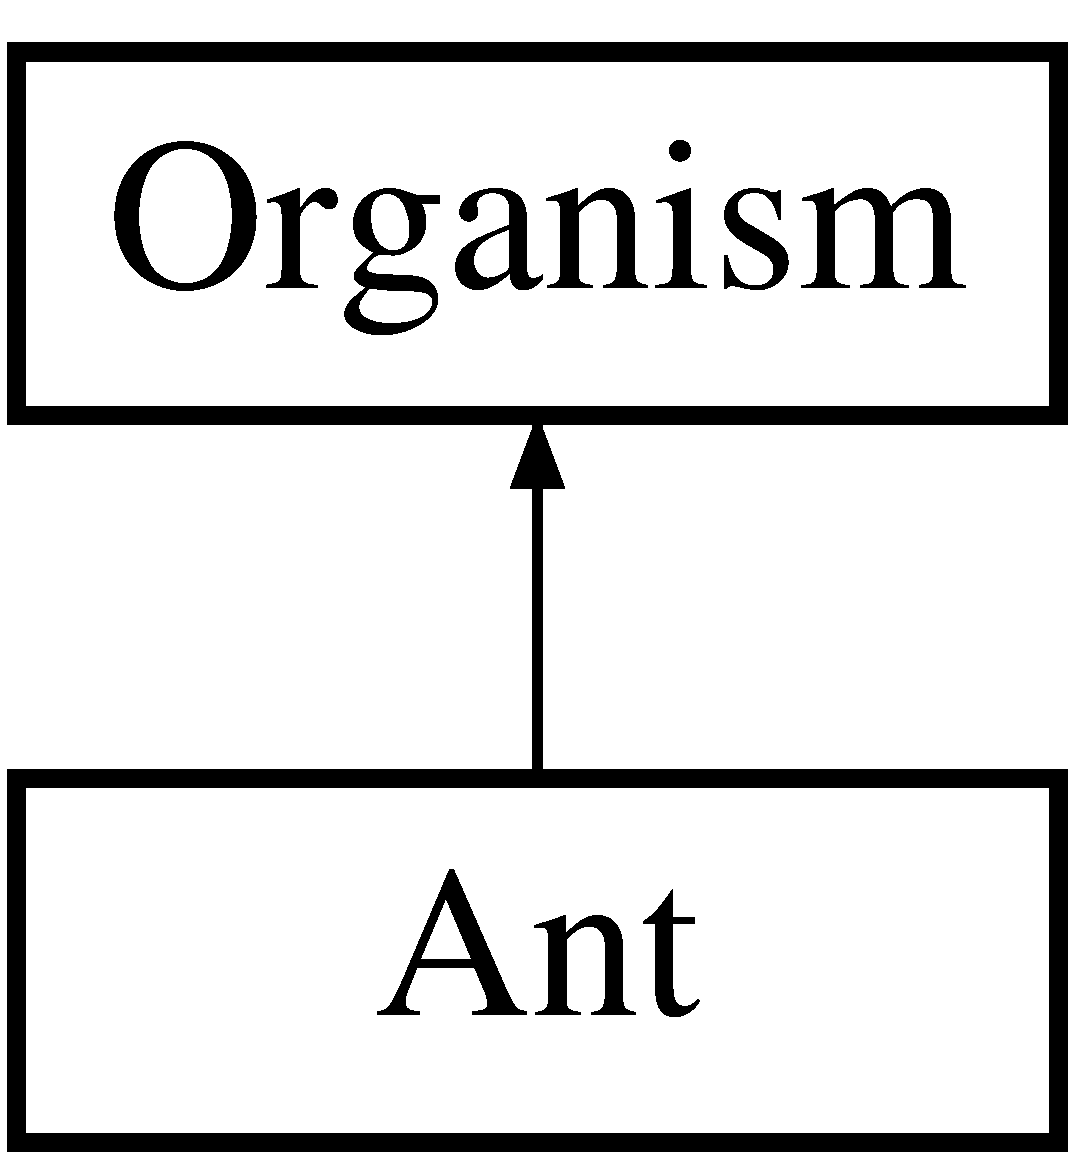
\includegraphics[height=2.000000cm]{classAnt}
\end{center}
\end{figure}
\subsection*{Public Member Functions}
\begin{DoxyCompactItemize}
\item 
\textbf{ Ant} ()
\item 
\textbf{ Ant} (int \textbf{ r}, int \textbf{ c}, \textbf{ Grid} $\ast$\textbf{ grid})
\item 
bool \textbf{ move} (\textbf{ Grid} $\ast$\textbf{ grid})
\item 
bool \textbf{ breed} (\textbf{ Grid} $\ast$\textbf{ grid})
\item 
void \textbf{ step} (\textbf{ Grid} $\ast$\textbf{ grid})
\item 
\textbf{ $\sim$\+Ant} ()
\end{DoxyCompactItemize}
\subsection*{Additional Inherited Members}


\subsection{Constructor \& Destructor Documentation}
\mbox{\label{classAnt_ad6c1a8f70419877f7a3e2c9c557f913d}} 
\index{Ant@{Ant}!Ant@{Ant}}
\index{Ant@{Ant}!Ant@{Ant}}
\subsubsection{Ant()\hspace{0.1cm}{\footnotesize\ttfamily [1/2]}}
{\footnotesize\ttfamily Ant\+::\+Ant (\begin{DoxyParamCaption}{ }\end{DoxyParamCaption})}

Default constructor for an \doxyref{Ant}{p.}{classAnt} object 

References Organism\+::c, Organism\+::grid, Organism\+::moves\+Without\+Breeding, and Organism\+::r.



Referenced by breed().

\mbox{\label{classAnt_ab9d3cd4e99035ed5dd479ca002af66d4}} 
\index{Ant@{Ant}!Ant@{Ant}}
\index{Ant@{Ant}!Ant@{Ant}}
\subsubsection{Ant()\hspace{0.1cm}{\footnotesize\ttfamily [2/2]}}
{\footnotesize\ttfamily Ant\+::\+Ant (\begin{DoxyParamCaption}\item[{int}]{r,  }\item[{int}]{c,  }\item[{\textbf{ Grid} $\ast$}]{grid }\end{DoxyParamCaption})}

Constructs an \doxyref{Ant}{p.}{classAnt} object at a certain location on the grid 
\begin{DoxyParams}{Parameters}
{\em r} & The row of the \doxyref{Ant}{p.}{classAnt} \\
\hline
{\em c} & the column of the \doxyref{Ant}{p.}{classAnt} \\
\hline
\end{DoxyParams}


References Organism\+::c, Organism\+::grid, Organism\+::moves\+Without\+Breeding, Organism\+::r, and Grid\+::set\+Cell\+Occupant().

\mbox{\label{classAnt_a33ca6bd592236726a18a2159908e4116}} 
\index{Ant@{Ant}!````~Ant@{$\sim$\+Ant}}
\index{````~Ant@{$\sim$\+Ant}!Ant@{Ant}}
\subsubsection{$\sim$\+Ant()}
{\footnotesize\ttfamily Ant\+::$\sim$\+Ant (\begin{DoxyParamCaption}{ }\end{DoxyParamCaption})}

Destructor for \doxyref{Ant}{p.}{classAnt} objects Clears memory formerly held by an \doxyref{Ant}{p.}{classAnt} 

References Organism\+::c, Organism\+::grid, Organism\+::r, and Grid\+::set\+Cell\+Occupant().



Referenced by Tests2\+::ants\+Die\+Test().



\subsection{Member Function Documentation}
\mbox{\label{classAnt_af899faded61186f5ca27e43cee1463ba}} 
\index{Ant@{Ant}!breed@{breed}}
\index{breed@{breed}!Ant@{Ant}}
\subsubsection{breed()}
{\footnotesize\ttfamily bool Ant\+::breed (\begin{DoxyParamCaption}\item[{\textbf{ Grid} $\ast$}]{grid }\end{DoxyParamCaption})\hspace{0.3cm}{\ttfamily [virtual]}}

Creates another \doxyref{Ant}{p.}{classAnt} object. If an \doxyref{Ant}{p.}{classAnt} survives three time steps, it will reproduce and create another \doxyref{Ant}{p.}{classAnt} in an adjacent cell. If no adjacent cells are available, the \doxyref{Ant}{p.}{classAnt} will wait until the next available turn to create another ant. If multiple adjacent cells are available, the \doxyref{Ant}{p.}{classAnt} will choose at random which adjacent cell it will create another \doxyref{Ant}{p.}{classAnt}. \begin{DoxyReturn}{Returns}
whether or not the \doxyref{Ant}{p.}{classAnt} was created successfully 
\end{DoxyReturn}


Implements \textbf{ Organism} \doxyref{}{p.}{classOrganism_a423246fb1dee94db6c8c3b08fba57ead}.



References Ant(), Organism\+::c, Organism\+::can\+Move\+Here(), Organism\+::moves\+Without\+Breeding, Grid\+::num\+Ants, Organism\+::r, and Grid\+::set\+Cell\+Occupant().



Referenced by Tests2\+::ants\+Breed\+Test(), Tests2\+::ants\+Dont\+Breed\+Test(), and step().

\mbox{\label{classAnt_a10d7a628d2459776b19d363a1fbf6dd9}} 
\index{Ant@{Ant}!move@{move}}
\index{move@{move}!Ant@{Ant}}
\subsubsection{move()}
{\footnotesize\ttfamily bool Ant\+::move (\begin{DoxyParamCaption}\item[{\textbf{ Grid} $\ast$}]{grid }\end{DoxyParamCaption})\hspace{0.3cm}{\ttfamily [virtual]}}

Moves the \doxyref{Ant}{p.}{classAnt} to a nearby cell. If the \doxyref{Ant}{p.}{classAnt} is surrounded by available adjacent cells (above, below, or to the left or right of the ant), it will move to one of these at random. If no cells are available, the \doxyref{Ant}{p.}{classAnt} will remain in the same location. \begin{DoxyReturn}{Returns}
Whether the \doxyref{Ant}{p.}{classAnt} moved successfully 
\end{DoxyReturn}


Implements \textbf{ Organism} \doxyref{}{p.}{classOrganism_a1f040ef71509bd11d302c50b168716f4}.



References Organism\+::c, Organism\+::can\+Move\+Here(), Organism\+::moves\+Without\+Breeding, Organism\+::r, and Grid\+::set\+Cell\+Occupant().



Referenced by Tests2\+::ants\+Dont\+Move\+Test(), Tests2\+::ants\+Move\+Test(), Tests2\+::doodle\+Eat\+Test(), and step().

\mbox{\label{classAnt_ada3517d6d55d5b69b82a028caa36ea1e}} 
\index{Ant@{Ant}!step@{step}}
\index{step@{step}!Ant@{Ant}}
\subsubsection{step()}
{\footnotesize\ttfamily void Ant\+::step (\begin{DoxyParamCaption}\item[{\textbf{ Grid} $\ast$}]{grid }\end{DoxyParamCaption})\hspace{0.3cm}{\ttfamily [virtual]}}

Causes the \doxyref{Ant}{p.}{classAnt} to take a step, i.\+e. move and/or breed 

Implements \textbf{ Organism} \doxyref{}{p.}{classOrganism_a4900481a90b69a85fe688cc1b962c9a2}.



References breed(), move(), and Organism\+::moves\+Without\+Breeding.



The documentation for this class was generated from the following files\+:\begin{DoxyCompactItemize}
\item 
\textbf{ Ant.\+h}\item 
\textbf{ Ant.\+cpp}\end{DoxyCompactItemize}

\section{Doodlebug Class Reference}
\label{classDoodlebug}\index{Doodlebug@{Doodlebug}}


{\ttfamily \#include $<$Doodlebug.\+h$>$}

Inheritance diagram for Doodlebug\+:\begin{figure}[H]
\begin{center}
\leavevmode
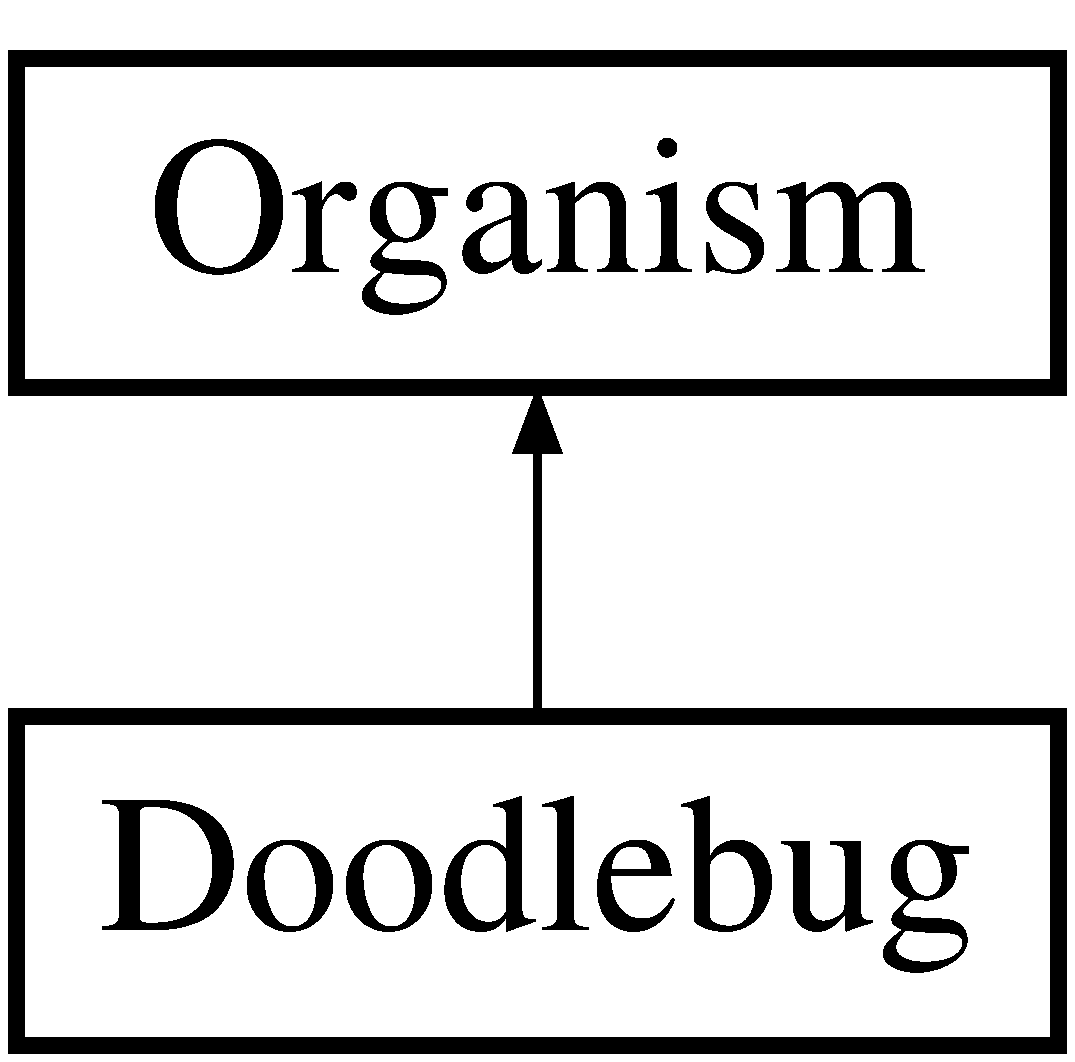
\includegraphics[height=2.000000cm]{classDoodlebug}
\end{center}
\end{figure}
\subsection*{Public Member Functions}
\begin{DoxyCompactItemize}
\item 
\textbf{ Doodlebug} ()
\item 
\textbf{ Doodlebug} (int \textbf{ r}, int \textbf{ c}, \textbf{ Grid} $\ast$\textbf{ grid})
\item 
bool \textbf{ move} (\textbf{ Grid} $\ast$\textbf{ grid})
\item 
bool \textbf{ breed} (\textbf{ Grid} $\ast$\textbf{ grid})
\item 
bool \textbf{ eat} (\textbf{ Grid} $\ast$\textbf{ grid}, int \textbf{ r}, int \textbf{ c})
\item 
void \textbf{ step} (\textbf{ Grid} $\ast$\textbf{ grid})
\item 
bool \textbf{ starve} ()
\item 
virtual \textbf{ $\sim$\+Doodlebug} ()
\end{DoxyCompactItemize}
\subsection*{Protected Attributes}
\begin{DoxyCompactItemize}
\item 
int \textbf{ steps\+Til\+Starve}
\end{DoxyCompactItemize}


\subsection{Constructor \& Destructor Documentation}
\mbox{\label{classDoodlebug_afb2796ea39a6ffa13d4f54ac68dd52fc}} 
\index{Doodlebug@{Doodlebug}!Doodlebug@{Doodlebug}}
\index{Doodlebug@{Doodlebug}!Doodlebug@{Doodlebug}}
\subsubsection{Doodlebug()\hspace{0.1cm}{\footnotesize\ttfamily [1/2]}}
{\footnotesize\ttfamily Doodlebug\+::\+Doodlebug (\begin{DoxyParamCaption}{ }\end{DoxyParamCaption})}

Default constructor for a \doxyref{Doodlebug}{p.}{classDoodlebug} object 

References Organism\+::c, Organism\+::grid, Organism\+::moves\+Without\+Breeding, Organism\+::r, and steps\+Til\+Starve.



Referenced by breed().

\mbox{\label{classDoodlebug_abd627e37a081281ab9e710c1e43829f4}} 
\index{Doodlebug@{Doodlebug}!Doodlebug@{Doodlebug}}
\index{Doodlebug@{Doodlebug}!Doodlebug@{Doodlebug}}
\subsubsection{Doodlebug()\hspace{0.1cm}{\footnotesize\ttfamily [2/2]}}
{\footnotesize\ttfamily Doodlebug\+::\+Doodlebug (\begin{DoxyParamCaption}\item[{int}]{r,  }\item[{int}]{c,  }\item[{\textbf{ Grid} $\ast$}]{grid }\end{DoxyParamCaption})}

Default constructor for a \doxyref{Doodlebug}{p.}{classDoodlebug} object which has row r and column c 
\begin{DoxyParams}{Parameters}
{\em r} & The row of the doodlebug \\
\hline
{\em c} & The column of the doodlebug \\
\hline
\end{DoxyParams}


References Organism\+::c, Grid\+::get\+Cell\+Occupant(), Organism\+::grid, Organism\+::moves\+Without\+Breeding, Organism\+::r, Organism\+::set\+Am\+Ant(), Grid\+::set\+Cell\+Occupant(), and steps\+Til\+Starve.

\mbox{\label{classDoodlebug_ac318cc9acbd9a3af52348a236070d891}} 
\index{Doodlebug@{Doodlebug}!````~Doodlebug@{$\sim$\+Doodlebug}}
\index{````~Doodlebug@{$\sim$\+Doodlebug}!Doodlebug@{Doodlebug}}
\subsubsection{$\sim$\+Doodlebug()}
{\footnotesize\ttfamily Doodlebug\+::$\sim$\+Doodlebug (\begin{DoxyParamCaption}{ }\end{DoxyParamCaption})\hspace{0.3cm}{\ttfamily [virtual]}}

Default destructor method for a \doxyref{Doodlebug}{p.}{classDoodlebug} Removes the \doxyref{Doodlebug}{p.}{classDoodlebug} from the board and from its space held in memory 

References Organism\+::c, Organism\+::grid, Organism\+::r, and Grid\+::set\+Cell\+Occupant().



Referenced by Tests2\+::doodle\+Dietest().



\subsection{Member Function Documentation}
\mbox{\label{classDoodlebug_a6ab3919da6f9404f1f3af05f0bbde13c}} 
\index{Doodlebug@{Doodlebug}!breed@{breed}}
\index{breed@{breed}!Doodlebug@{Doodlebug}}
\subsubsection{breed()}
{\footnotesize\ttfamily bool Doodlebug\+::breed (\begin{DoxyParamCaption}\item[{\textbf{ Grid} $\ast$}]{grid }\end{DoxyParamCaption})\hspace{0.3cm}{\ttfamily [virtual]}}

Creates another \doxyref{Doodlebug}{p.}{classDoodlebug} object. If a \doxyref{Doodlebug}{p.}{classDoodlebug} survives eight time steps, it will reproduce and create another \doxyref{Doodlebug}{p.}{classDoodlebug} in an adjacent cell. If no adjacent cells are available, the \doxyref{Doodlebug}{p.}{classDoodlebug} will wait until the next available turn to create another \doxyref{Doodlebug}{p.}{classDoodlebug}. If multiple adjacent cells are available, the \doxyref{Doodlebug}{p.}{classDoodlebug} will choose at random which adjacent cell it will create another \doxyref{Doodlebug}{p.}{classDoodlebug}. \begin{DoxyReturn}{Returns}
whether or not the \doxyref{Doodlebug}{p.}{classDoodlebug} was created successfully 
\end{DoxyReturn}


Implements \textbf{ Organism} \doxyref{}{p.}{classOrganism_a423246fb1dee94db6c8c3b08fba57ead}.



References Organism\+::c, Organism\+::can\+Move\+Here(), Doodlebug(), Organism\+::moves\+Without\+Breeding, Grid\+::num\+Doodlebugs, Organism\+::r, and Grid\+::set\+Cell\+Occupant().



Referenced by Tests2\+::doodle\+Breed\+Test(), Tests2\+::doodle\+Dont\+Breed\+Test(), and step().

\mbox{\label{classDoodlebug_aface39c7df1602eff9830a6c3e0a973a}} 
\index{Doodlebug@{Doodlebug}!eat@{eat}}
\index{eat@{eat}!Doodlebug@{Doodlebug}}
\subsubsection{eat()}
{\footnotesize\ttfamily bool Doodlebug\+::eat (\begin{DoxyParamCaption}\item[{\textbf{ Grid} $\ast$}]{grid,  }\item[{int}]{r,  }\item[{int}]{c }\end{DoxyParamCaption})}

Consumes an \doxyref{Ant}{p.}{classAnt}, moving into its space and removing it from the board 
\begin{DoxyParams}{Parameters}
{\em grid} & The home grid for the doodlebug \\
\hline
{\em r} & The row of the \doxyref{Ant}{p.}{classAnt} \\
\hline
{\em c} & The column of the \doxyref{Ant}{p.}{classAnt} \\
\hline
\end{DoxyParams}
\begin{DoxyReturn}{Returns}
Whether or not the \doxyref{Ant}{p.}{classAnt} was eaten successfully 
\end{DoxyReturn}


References Grid\+::get\+Cell\+Occupant(), Grid\+::num\+Ants, Grid\+::set\+Cell\+Occupant(), and steps\+Til\+Starve.



Referenced by Tests2\+::doodle\+Eat\+Test(), and move().

\mbox{\label{classDoodlebug_a4f00da3e326d355a66e936110ce70f15}} 
\index{Doodlebug@{Doodlebug}!move@{move}}
\index{move@{move}!Doodlebug@{Doodlebug}}
\subsubsection{move()}
{\footnotesize\ttfamily bool Doodlebug\+::move (\begin{DoxyParamCaption}\item[{\textbf{ Grid} $\ast$}]{grid }\end{DoxyParamCaption})\hspace{0.3cm}{\ttfamily [virtual]}}

Moves the \doxyref{Doodlebug}{p.}{classDoodlebug} to a nearby cell, usually so that it can eat an \doxyref{Ant}{p.}{classAnt} If a \doxyref{Doodlebug}{p.}{classDoodlebug} is adjacent to an \doxyref{Ant}{p.}{classAnt} (above, below, or to the left or right of the ant), it will move to the Cell of the \doxyref{Ant}{p.}{classAnt} at random and eat it. If no Ants are nearby, the \doxyref{Doodlebug}{p.}{classDoodlebug} will move according to the rules of an \doxyref{Ant}{p.}{classAnt} moving. If the \doxyref{Doodlebug}{p.}{classDoodlebug} has not eaten any Ants for three time steps, it will die of starvation at the end of the third time step. If no Cells are available, the \doxyref{Doodlebug}{p.}{classDoodlebug} will remain in the same location. \begin{DoxyReturn}{Returns}
Whether the \doxyref{Doodlebug}{p.}{classDoodlebug} moved successfully 
\end{DoxyReturn}


Implements \textbf{ Organism} \doxyref{}{p.}{classOrganism_a1f040ef71509bd11d302c50b168716f4}.



References Organism\+::c, Organism\+::can\+Move\+Here(), Organism\+::doodle\+Can\+Move\+Here(), eat(), Grid\+::get\+Cell\+Occupant(), Organism\+::is\+Prey(), Organism\+::moves\+Without\+Breeding, Grid\+::n, Organism\+::r, Grid\+::set\+Cell\+Occupant(), and steps\+Til\+Starve.



Referenced by Tests2\+::doodle\+Dont\+Move\+Test(), Tests2\+::doodle\+Move\+Test(), and step().

\mbox{\label{classDoodlebug_a7f1c26c8458f3811680c778362c0e374}} 
\index{Doodlebug@{Doodlebug}!starve@{starve}}
\index{starve@{starve}!Doodlebug@{Doodlebug}}
\subsubsection{starve()}
{\footnotesize\ttfamily bool Doodlebug\+::starve (\begin{DoxyParamCaption}{ }\end{DoxyParamCaption})}

Checks whether the \doxyref{Doodlebug}{p.}{classDoodlebug} will starve \begin{DoxyReturn}{Returns}
true if the \doxyref{Doodlebug}{p.}{classDoodlebug} starved, false otherwise 
\end{DoxyReturn}


References steps\+Til\+Starve.



Referenced by step().

\mbox{\label{classDoodlebug_a92f534cbd8df9342c324ccf240440f11}} 
\index{Doodlebug@{Doodlebug}!step@{step}}
\index{step@{step}!Doodlebug@{Doodlebug}}
\subsubsection{step()}
{\footnotesize\ttfamily void Doodlebug\+::step (\begin{DoxyParamCaption}\item[{\textbf{ Grid} $\ast$}]{grid }\end{DoxyParamCaption})\hspace{0.3cm}{\ttfamily [virtual]}}

Causes the \doxyref{Doodlebug}{p.}{classDoodlebug} to take a step, i.\+e. move and/or breed 

Implements \textbf{ Organism} \doxyref{}{p.}{classOrganism_a4900481a90b69a85fe688cc1b962c9a2}.



References breed(), move(), Organism\+::moves\+Without\+Breeding, Grid\+::num\+Doodlebugs, and starve().



\subsection{Field Documentation}
\mbox{\label{classDoodlebug_a3afff57dedcacfbcbf1cdc5c877844a5}} 
\index{Doodlebug@{Doodlebug}!steps\+Til\+Starve@{steps\+Til\+Starve}}
\index{steps\+Til\+Starve@{steps\+Til\+Starve}!Doodlebug@{Doodlebug}}
\subsubsection{steps\+Til\+Starve}
{\footnotesize\ttfamily int Doodlebug\+::steps\+Til\+Starve\hspace{0.3cm}{\ttfamily [protected]}}



Referenced by Doodlebug(), eat(), move(), and starve().



The documentation for this class was generated from the following files\+:\begin{DoxyCompactItemize}
\item 
\textbf{ Doodlebug.\+h}\item 
\textbf{ Doodlebug.\+cpp}\end{DoxyCompactItemize}

\section{Grid Class Reference}
\label{classGrid}\index{Grid@{Grid}}


{\ttfamily \#include $<$Grid.\+h$>$}

\subsection*{Public Member Functions}
\begin{DoxyCompactItemize}
\item 
\textbf{ Grid} ()
\item 
\textbf{ Grid} (int n\+Squares\+On\+A\+Side, int num\+Doodles, int \textbf{ num\+Ants})
\item 
void \textbf{ set\+Cell\+Occupant} (int r, int c, \textbf{ Organism} $\ast$o)
\item 
\textbf{ Organism} $\ast$ \textbf{ get\+Cell\+Occupant} (int r, int c)
\item 
void \textbf{ step} (int r, int c)
\item 
char \textbf{ get\+Letter} (int r, int c)
\item 
void \textbf{ print\+Grid} ()
\item 
void \textbf{ randomize\+Grid} (int R\+NG)
\item 
virtual \textbf{ $\sim$\+Grid} ()
\end{DoxyCompactItemize}
\subsection*{Data Fields}
\begin{DoxyCompactItemize}
\item 
int \textbf{ num\+Ants}
\item 
int \textbf{ num\+Doodlebugs}
\item 
\textbf{ Organism} $\ast$$\ast$$\ast$ \textbf{ org\+Array} = (\textbf{ Organism}$\ast$$\ast$$\ast$)nullptr
\item 
int \textbf{ n} =0
\end{DoxyCompactItemize}


\subsection{Constructor \& Destructor Documentation}
\mbox{\label{classGrid_a4ac9ff4f63552b4c61ff90fcb35ad66c}} 
\index{Grid@{Grid}!Grid@{Grid}}
\index{Grid@{Grid}!Grid@{Grid}}
\subsubsection{Grid()\hspace{0.1cm}{\footnotesize\ttfamily [1/2]}}
{\footnotesize\ttfamily Grid\+::\+Grid (\begin{DoxyParamCaption}{ }\end{DoxyParamCaption})}

Creates a \doxyref{Grid}{p.}{classGrid} of a default number of Cells 

References n, num\+Ants, num\+Doodlebugs, and org\+Array.

\mbox{\label{classGrid_a68475d9701f21e276b297126126cdc10}} 
\index{Grid@{Grid}!Grid@{Grid}}
\index{Grid@{Grid}!Grid@{Grid}}
\subsubsection{Grid()\hspace{0.1cm}{\footnotesize\ttfamily [2/2]}}
{\footnotesize\ttfamily Grid\+::\+Grid (\begin{DoxyParamCaption}\item[{int}]{n\+Squares\+On\+A\+Side,  }\item[{int}]{num\+Doodlebugs,  }\item[{int}]{num\+Ants }\end{DoxyParamCaption})}

Creates a \doxyref{Grid}{p.}{classGrid} with a given number of Cells on each side 
\begin{DoxyParams}{Parameters}
{\em n\+Squares\+On\+A\+Side} & The amount of squares on each side of the board \\
\hline
\end{DoxyParams}


References n, num\+Ants, num\+Doodlebugs, and org\+Array.

\mbox{\label{classGrid_a3661d0a7f998caaaf8627d7a67072116}} 
\index{Grid@{Grid}!````~Grid@{$\sim$\+Grid}}
\index{````~Grid@{$\sim$\+Grid}!Grid@{Grid}}
\subsubsection{$\sim$\+Grid()}
{\footnotesize\ttfamily Grid\+::$\sim$\+Grid (\begin{DoxyParamCaption}{ }\end{DoxyParamCaption})\hspace{0.3cm}{\ttfamily [virtual]}}

Destroys the given \doxyref{Grid}{p.}{classGrid}, going row by row and removing each Cell from memory 

References n, and org\+Array.



\subsection{Member Function Documentation}
\mbox{\label{classGrid_a42fb1a75c9cf52ca8c92014d38abfc88}} 
\index{Grid@{Grid}!get\+Cell\+Occupant@{get\+Cell\+Occupant}}
\index{get\+Cell\+Occupant@{get\+Cell\+Occupant}!Grid@{Grid}}
\subsubsection{get\+Cell\+Occupant()}
{\footnotesize\ttfamily \textbf{ Organism} $\ast$ Grid\+::get\+Cell\+Occupant (\begin{DoxyParamCaption}\item[{int}]{r,  }\item[{int}]{c }\end{DoxyParamCaption})}

Returns the occupant of a given Cell. Will not check if r and c are within bounds! 
\begin{DoxyParams}{Parameters}
{\em r} & the row of the given Cell \\
\hline
{\em c} & the column of the given Cell \\
\hline
\end{DoxyParams}
\begin{DoxyReturn}{Returns}
A pointer to the organism in the cell 
\end{DoxyReturn}


References org\+Array.



Referenced by Tests2\+::ants\+Breed\+Test(), Tests2\+::ants\+Die\+Test(), Tests2\+::ants\+Dont\+Breed\+Test(), Tests2\+::ants\+Dont\+Move\+Test(), Tests2\+::ants\+Move\+Test(), Organism\+::can\+Move\+Here(), Tests2\+::doodle\+Breed\+Test(), Doodlebug\+::\+Doodlebug(), Organism\+::doodle\+Can\+Move\+Here(), Tests2\+::doodle\+Dietest(), Tests2\+::doodle\+Dont\+Breed\+Test(), Tests2\+::doodle\+Dont\+Move\+Test(), Tests2\+::doodle\+Eat\+Test(), Tests2\+::doodle\+Move\+Test(), Doodlebug\+::eat(), Tests2\+::grid\+Test(), Organism\+::is\+Empty(), Tests2\+::make\+Ants\+Test(), Tests2\+::make\+Doodles\+Test(), Doodlebug\+::move(), randomize\+Grid(), and step().

\mbox{\label{classGrid_ae6ea956ae4568eb1fa3bb1b0cb7a0a39}} 
\index{Grid@{Grid}!get\+Letter@{get\+Letter}}
\index{get\+Letter@{get\+Letter}!Grid@{Grid}}
\subsubsection{get\+Letter()}
{\footnotesize\ttfamily char Grid\+::get\+Letter (\begin{DoxyParamCaption}\item[{int}]{r,  }\item[{int}]{c }\end{DoxyParamCaption})}

Returns a letter corresponding to the type of \doxyref{Organism}{p.}{classOrganism} in a certain Cell \begin{DoxyReturn}{Returns}
a letter that corresponds to the type of \doxyref{Organism}{p.}{classOrganism} in a certain Cell 
\end{DoxyReturn}


References org\+Array.



Referenced by print\+Grid().

\mbox{\label{classGrid_a04601ea9795a6928190e64fa89f10499}} 
\index{Grid@{Grid}!print\+Grid@{print\+Grid}}
\index{print\+Grid@{print\+Grid}!Grid@{Grid}}
\subsubsection{print\+Grid()}
{\footnotesize\ttfamily void Grid\+::print\+Grid (\begin{DoxyParamCaption}{ }\end{DoxyParamCaption})}

Prints out the grid in a format corresponding to what is in each Cell x if the organism is a \doxyref{Doodlebug}{p.}{classDoodlebug} o if the organism is an \doxyref{Ant}{p.}{classAnt} \textquotesingle{} \textquotesingle{} (empty space) if the cell is empty 
\begin{DoxyParams}{Parameters}
{\em grid} & The grid to be printed \\
\hline
{\em r} & The number of rows in the grid \\
\hline
{\em c} & The number of columns in the grid \\
\hline
\end{DoxyParams}


References get\+Letter(), and n.



Referenced by Tests2\+::ants\+Breed\+Test(), Tests2\+::ants\+Die\+Test(), Tests2\+::ants\+Dont\+Breed\+Test(), Tests2\+::ants\+Dont\+Move\+Test(), Tests2\+::ants\+Move\+Test(), Tests2\+::doodle\+Breed\+Test(), Tests2\+::doodle\+Dietest(), Tests2\+::doodle\+Dont\+Breed\+Test(), Tests2\+::doodle\+Dont\+Move\+Test(), Tests2\+::doodle\+Eat\+Test(), Tests2\+::doodle\+Move\+Test(), Tests2\+::grid\+Test(), Tests2\+::make\+Ants\+Test(), Tests2\+::make\+Doodles\+Test(), and Production\+::run\+Production().

\mbox{\label{classGrid_a3d34142ead519cb09d47d6f87f77f863}} 
\index{Grid@{Grid}!randomize\+Grid@{randomize\+Grid}}
\index{randomize\+Grid@{randomize\+Grid}!Grid@{Grid}}
\subsubsection{randomize\+Grid()}
{\footnotesize\ttfamily void Grid\+::randomize\+Grid (\begin{DoxyParamCaption}\item[{int}]{R\+NG }\end{DoxyParamCaption})}

Fills org\+Array with random Organisms based on the number of each count 

References get\+Cell\+Occupant(), n, num\+Ants, num\+Doodlebugs, and set\+Cell\+Occupant().



Referenced by Production\+::run\+Production().

\mbox{\label{classGrid_a0f63830487262e45858a8ea451e341f2}} 
\index{Grid@{Grid}!set\+Cell\+Occupant@{set\+Cell\+Occupant}}
\index{set\+Cell\+Occupant@{set\+Cell\+Occupant}!Grid@{Grid}}
\subsubsection{set\+Cell\+Occupant()}
{\footnotesize\ttfamily void Grid\+::set\+Cell\+Occupant (\begin{DoxyParamCaption}\item[{int}]{r,  }\item[{int}]{c,  }\item[{\textbf{ Organism} $\ast$}]{o }\end{DoxyParamCaption})}

Sets the occupant of the cell to the given values. 
\begin{DoxyParams}{Parameters}
{\em r} & The row of the occupant \\
\hline
{\em c} & The column of the occupant \\
\hline
{\em g} & The new occupant \\
\hline
\end{DoxyParams}


References org\+Array.



Referenced by Ant\+::\+Ant(), Ant\+::breed(), Doodlebug\+::breed(), Doodlebug\+::\+Doodlebug(), Doodlebug\+::eat(), Tests2\+::grid\+Test(), Tests2\+::make\+Ants\+Test(), Ant\+::move(), Doodlebug\+::move(), randomize\+Grid(), Ant\+::$\sim$\+Ant(), Doodlebug\+::$\sim$\+Doodlebug(), and Organism\+::$\sim$\+Organism().

\mbox{\label{classGrid_a13c2a8c9eddcb7f5933f3d7c16a06d6c}} 
\index{Grid@{Grid}!step@{step}}
\index{step@{step}!Grid@{Grid}}
\subsubsection{step()}
{\footnotesize\ttfamily void Grid\+::step (\begin{DoxyParamCaption}\item[{int}]{r,  }\item[{int}]{c }\end{DoxyParamCaption})}

Takes one \char`\"{}step\char`\"{} through the game. 

References get\+Cell\+Occupant(), org\+Array, and Organism\+::step().



Referenced by Production\+::run\+Production().



\subsection{Field Documentation}
\mbox{\label{classGrid_a9a0956abaf6071329601a9dc9c9e706c}} 
\index{Grid@{Grid}!n@{n}}
\index{n@{n}!Grid@{Grid}}
\subsubsection{n}
{\footnotesize\ttfamily int Grid\+::n =0}



Referenced by Organism\+::can\+Move\+Here(), Organism\+::doodle\+Can\+Move\+Here(), Grid(), Doodlebug\+::move(), print\+Grid(), randomize\+Grid(), and $\sim$\+Grid().

\mbox{\label{classGrid_a057a3f91bbaf94d7756d17c56fcedbea}} 
\index{Grid@{Grid}!num\+Ants@{num\+Ants}}
\index{num\+Ants@{num\+Ants}!Grid@{Grid}}
\subsubsection{num\+Ants}
{\footnotesize\ttfamily int Grid\+::num\+Ants}



Referenced by Ant\+::breed(), Doodlebug\+::eat(), Grid(), randomize\+Grid(), and Production\+::run\+Production().

\mbox{\label{classGrid_ae9ebdf747bc46ca69c502eb56c984f33}} 
\index{Grid@{Grid}!num\+Doodlebugs@{num\+Doodlebugs}}
\index{num\+Doodlebugs@{num\+Doodlebugs}!Grid@{Grid}}
\subsubsection{num\+Doodlebugs}
{\footnotesize\ttfamily int Grid\+::num\+Doodlebugs}



Referenced by Doodlebug\+::breed(), Grid(), randomize\+Grid(), Production\+::run\+Production(), and Doodlebug\+::step().

\mbox{\label{classGrid_a785e43fc15bcc03b163e9f42140c1aa3}} 
\index{Grid@{Grid}!org\+Array@{org\+Array}}
\index{org\+Array@{org\+Array}!Grid@{Grid}}
\subsubsection{org\+Array}
{\footnotesize\ttfamily \textbf{ Organism}$\ast$$\ast$$\ast$ Grid\+::org\+Array = (\textbf{ Organism}$\ast$$\ast$$\ast$)nullptr}



Referenced by get\+Cell\+Occupant(), get\+Letter(), Grid(), set\+Cell\+Occupant(), step(), and $\sim$\+Grid().



The documentation for this class was generated from the following files\+:\begin{DoxyCompactItemize}
\item 
\textbf{ Grid.\+h}\item 
\textbf{ Grid.\+cpp}\end{DoxyCompactItemize}

\section{Organism Class Reference}
\label{classOrganism}\index{Organism@{Organism}}


{\ttfamily \#include $<$Organism.\+h$>$}

Inheritance diagram for Organism\+:\begin{figure}[H]
\begin{center}
\leavevmode
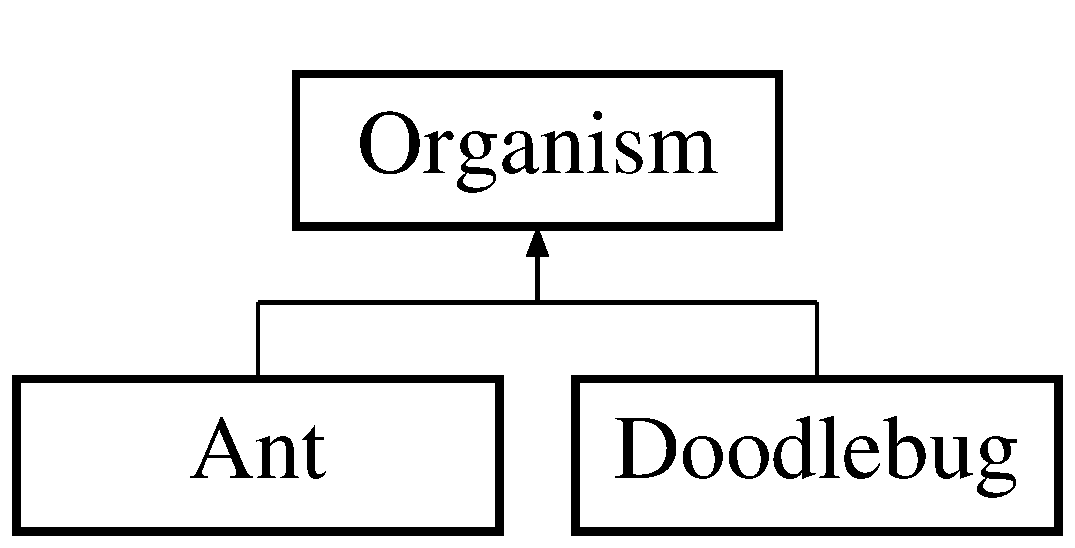
\includegraphics[height=2.000000cm]{classOrganism}
\end{center}
\end{figure}
\subsection*{Public Member Functions}
\begin{DoxyCompactItemize}
\item 
\textbf{ Organism} ()
\item 
\textbf{ Organism} (bool b)
\item 
bool \textbf{ is\+Prey} ()
\item 
virtual bool \textbf{ move} (\textbf{ Grid} $\ast$\textbf{ grid})=0
\item 
virtual bool \textbf{ breed} (\textbf{ Grid} $\ast$\textbf{ grid})=0
\item 
virtual void \textbf{ step} (\textbf{ Grid} $\ast$\textbf{ grid})=0
\item 
bool \textbf{ check\+Empty\+Spaces} (\textbf{ Grid} $\ast$\textbf{ grid}, int \textbf{ r}, int \textbf{ c})
\item 
bool \textbf{ is\+Empty} (\textbf{ Grid} $\ast$\textbf{ grid}, int \textbf{ r}, int \textbf{ c})
\item 
void \textbf{ set\+Am\+Ant} (bool b)
\item 
bool \textbf{ can\+Move\+Here} (int direction, \textbf{ Grid} $\ast$g, int \textbf{ r}, int \textbf{ c})
\item 
bool \textbf{ doodle\+Can\+Move\+Here} (int direction, \textbf{ Grid} $\ast$g, int \textbf{ r}, int \textbf{ c})
\item 
virtual \textbf{ $\sim$\+Organism} ()
\end{DoxyCompactItemize}
\subsection*{Protected Attributes}
\begin{DoxyCompactItemize}
\item 
bool \textbf{ am\+Ant} = true
\item 
int \textbf{ r}
\item 
int \textbf{ c}
\item 
int \textbf{ moves\+Without\+Breeding}
\item 
\textbf{ Grid} $\ast$ \textbf{ grid}
\end{DoxyCompactItemize}


\subsection{Constructor \& Destructor Documentation}
\mbox{\label{classOrganism_aeb16ee24b64839584b4862384d0b53fe}} 
\index{Organism@{Organism}!Organism@{Organism}}
\index{Organism@{Organism}!Organism@{Organism}}
\subsubsection{Organism()\hspace{0.1cm}{\footnotesize\ttfamily [1/2]}}
{\footnotesize\ttfamily Organism\+::\+Organism (\begin{DoxyParamCaption}{ }\end{DoxyParamCaption})}

Default constructor for an \doxyref{Organism}{p.}{classOrganism} 

References c, grid, moves\+Without\+Breeding, and r.

\mbox{\label{classOrganism_ac7d3dbebaf5df39d0a7883b2d76b4868}} 
\index{Organism@{Organism}!Organism@{Organism}}
\index{Organism@{Organism}!Organism@{Organism}}
\subsubsection{Organism()\hspace{0.1cm}{\footnotesize\ttfamily [2/2]}}
{\footnotesize\ttfamily Organism\+::\+Organism (\begin{DoxyParamCaption}\item[{bool}]{b }\end{DoxyParamCaption})}

Constructor for an \doxyref{Organism}{p.}{classOrganism}, which may or may not be an \doxyref{Ant}{p.}{classAnt} 
\begin{DoxyParams}{Parameters}
{\em b} & Whether or not the \doxyref{Organism}{p.}{classOrganism} is an \doxyref{Ant}{p.}{classAnt} \\
\hline
\end{DoxyParams}


References am\+Ant, c, grid, moves\+Without\+Breeding, and r.

\mbox{\label{classOrganism_aa5aa2e9fc3134358c929fa0c9d230c3b}} 
\index{Organism@{Organism}!````~Organism@{$\sim$\+Organism}}
\index{````~Organism@{$\sim$\+Organism}!Organism@{Organism}}
\subsubsection{$\sim$\+Organism()}
{\footnotesize\ttfamily Organism\+::$\sim$\+Organism (\begin{DoxyParamCaption}{ }\end{DoxyParamCaption})\hspace{0.3cm}{\ttfamily [virtual]}}

Destructor for an \doxyref{Organism}{p.}{classOrganism} Removes the \doxyref{Organism}{p.}{classOrganism} from the \doxyref{Grid}{p.}{classGrid} and memory 

References c, grid, r, and Grid\+::set\+Cell\+Occupant().



\subsection{Member Function Documentation}
\mbox{\label{classOrganism_a423246fb1dee94db6c8c3b08fba57ead}} 
\index{Organism@{Organism}!breed@{breed}}
\index{breed@{breed}!Organism@{Organism}}
\subsubsection{breed()}
{\footnotesize\ttfamily virtual bool Organism\+::breed (\begin{DoxyParamCaption}\item[{\textbf{ Grid} $\ast$}]{grid }\end{DoxyParamCaption})\hspace{0.3cm}{\ttfamily [pure virtual]}}



Implemented in \textbf{ Doodlebug} \doxyref{}{p.}{classDoodlebug_a6ab3919da6f9404f1f3af05f0bbde13c}, and \textbf{ Ant} \doxyref{}{p.}{classAnt_af899faded61186f5ca27e43cee1463ba}.

\mbox{\label{classOrganism_abd7d82fe6ef801008c9f1fb5ca25e0a4}} 
\index{Organism@{Organism}!can\+Move\+Here@{can\+Move\+Here}}
\index{can\+Move\+Here@{can\+Move\+Here}!Organism@{Organism}}
\subsubsection{can\+Move\+Here()}
{\footnotesize\ttfamily bool Organism\+::can\+Move\+Here (\begin{DoxyParamCaption}\item[{int}]{direction,  }\item[{\textbf{ Grid} $\ast$}]{g,  }\item[{int}]{r,  }\item[{int}]{c }\end{DoxyParamCaption})}

Checks if the organism is able to move in the direction specified by direction. direction follows cardinal directions, i.\+e. 0 = north, 1 = east 2 = south, 3 = west Different from is\+Empty because it checks whether the given space is within the bounds of the grid. 
\begin{DoxyParams}{Parameters}
{\em direction} & The cardinal direction that the organism will be moving in \\
\hline
{\em g} & The grid that will be checked \\
\hline
{\em r} & The row of the organism \\
\hline
{\em c} & The column of the organism \\
\hline
\end{DoxyParams}
\begin{DoxyReturn}{Returns}
true if the organism can move to this space, false otherwise 
\end{DoxyReturn}


References Grid\+::get\+Cell\+Occupant(), is\+Empty(), and Grid\+::n.



Referenced by Ant\+::breed(), Doodlebug\+::breed(), Ant\+::move(), and Doodlebug\+::move().

\mbox{\label{classOrganism_a6248dae43f8697249e8db859c21b2b4c}} 
\index{Organism@{Organism}!check\+Empty\+Spaces@{check\+Empty\+Spaces}}
\index{check\+Empty\+Spaces@{check\+Empty\+Spaces}!Organism@{Organism}}
\subsubsection{check\+Empty\+Spaces()}
{\footnotesize\ttfamily bool Organism\+::check\+Empty\+Spaces (\begin{DoxyParamCaption}\item[{\textbf{ Grid} $\ast$}]{grid,  }\item[{int}]{r,  }\item[{int}]{c }\end{DoxyParamCaption})}

\mbox{\label{classOrganism_aa699fff3a6b00c93e8b6070c299342c0}} 
\index{Organism@{Organism}!doodle\+Can\+Move\+Here@{doodle\+Can\+Move\+Here}}
\index{doodle\+Can\+Move\+Here@{doodle\+Can\+Move\+Here}!Organism@{Organism}}
\subsubsection{doodle\+Can\+Move\+Here()}
{\footnotesize\ttfamily bool Organism\+::doodle\+Can\+Move\+Here (\begin{DoxyParamCaption}\item[{int}]{direction,  }\item[{\textbf{ Grid} $\ast$}]{g,  }\item[{int}]{r,  }\item[{int}]{c }\end{DoxyParamCaption})}

Checks if the doodlebug is able to move in the direction specified by direction. direction follows cardinal directions, i.\+e. 0 = north, 1 = east 2 = south, 3 = west Different from is\+Empty because it checks whether the given space is within the bounds of the grid. Different from can\+Move\+Here because it checks whether or not the space is occupied by an ant 
\begin{DoxyParams}{Parameters}
{\em direction} & The cardinal direction that the organism will be moving in \\
\hline
{\em g} & The grid that will be checked \\
\hline
{\em r} & The row of the organism \\
\hline
{\em c} & The column of the organism \\
\hline
\end{DoxyParams}
\begin{DoxyReturn}{Returns}
true if the doodlebug can move to this space, false otherwise 
\end{DoxyReturn}


References Grid\+::get\+Cell\+Occupant(), is\+Prey(), and Grid\+::n.



Referenced by Doodlebug\+::move().

\mbox{\label{classOrganism_a2b171e4babfb65d2ed18544f713ec8ee}} 
\index{Organism@{Organism}!is\+Empty@{is\+Empty}}
\index{is\+Empty@{is\+Empty}!Organism@{Organism}}
\subsubsection{is\+Empty()}
{\footnotesize\ttfamily bool Organism\+::is\+Empty (\begin{DoxyParamCaption}\item[{\textbf{ Grid} $\ast$}]{grid,  }\item[{int}]{r,  }\item[{int}]{c }\end{DoxyParamCaption})}

Checks whether or not the given Cell is occupied by something. 
\begin{DoxyParams}{Parameters}
{\em grid} & The grid that will be checked \\
\hline
\end{DoxyParams}
\begin{DoxyReturn}{Returns}
true if there is nothing in the given space, false otherwise 
\end{DoxyReturn}


References Grid\+::get\+Cell\+Occupant().



Referenced by can\+Move\+Here().

\mbox{\label{classOrganism_aa5213b2e2b0c4f227dc7dfc4c4ab411c}} 
\index{Organism@{Organism}!is\+Prey@{is\+Prey}}
\index{is\+Prey@{is\+Prey}!Organism@{Organism}}
\subsubsection{is\+Prey()}
{\footnotesize\ttfamily bool Organism\+::is\+Prey (\begin{DoxyParamCaption}{ }\end{DoxyParamCaption})}

Whether or not the \doxyref{Organism}{p.}{classOrganism} is an \doxyref{Ant}{p.}{classAnt} \begin{DoxyReturn}{Returns}
true if the \doxyref{Organism}{p.}{classOrganism} is an \doxyref{Ant}{p.}{classAnt} or nullptr false if the \doxyref{Organism}{p.}{classOrganism} is not an \doxyref{Ant}{p.}{classAnt} 
\end{DoxyReturn}


References am\+Ant.



Referenced by doodle\+Can\+Move\+Here(), and Doodlebug\+::move().

\mbox{\label{classOrganism_a1f040ef71509bd11d302c50b168716f4}} 
\index{Organism@{Organism}!move@{move}}
\index{move@{move}!Organism@{Organism}}
\subsubsection{move()}
{\footnotesize\ttfamily virtual bool Organism\+::move (\begin{DoxyParamCaption}\item[{\textbf{ Grid} $\ast$}]{grid }\end{DoxyParamCaption})\hspace{0.3cm}{\ttfamily [pure virtual]}}



Implemented in \textbf{ Doodlebug} \doxyref{}{p.}{classDoodlebug_a4f00da3e326d355a66e936110ce70f15}, and \textbf{ Ant} \doxyref{}{p.}{classAnt_a10d7a628d2459776b19d363a1fbf6dd9}.

\mbox{\label{classOrganism_aba68f4745f6b0938cf157dcd27df1868}} 
\index{Organism@{Organism}!set\+Am\+Ant@{set\+Am\+Ant}}
\index{set\+Am\+Ant@{set\+Am\+Ant}!Organism@{Organism}}
\subsubsection{set\+Am\+Ant()}
{\footnotesize\ttfamily void Organism\+::set\+Am\+Ant (\begin{DoxyParamCaption}\item[{bool}]{b }\end{DoxyParamCaption})}

Sets the status of an \doxyref{Organism}{p.}{classOrganism} to being an \doxyref{Ant}{p.}{classAnt} or not being an \doxyref{Ant}{p.}{classAnt} 
\begin{DoxyParams}{Parameters}
{\em b} & Whether or not the \doxyref{Organism}{p.}{classOrganism} is an \doxyref{Ant}{p.}{classAnt} \\
\hline
\end{DoxyParams}


References am\+Ant.



Referenced by Doodlebug\+::\+Doodlebug().

\mbox{\label{classOrganism_a4900481a90b69a85fe688cc1b962c9a2}} 
\index{Organism@{Organism}!step@{step}}
\index{step@{step}!Organism@{Organism}}
\subsubsection{step()}
{\footnotesize\ttfamily virtual void Organism\+::step (\begin{DoxyParamCaption}\item[{\textbf{ Grid} $\ast$}]{grid }\end{DoxyParamCaption})\hspace{0.3cm}{\ttfamily [pure virtual]}}



Implemented in \textbf{ Doodlebug} \doxyref{}{p.}{classDoodlebug_a92f534cbd8df9342c324ccf240440f11}, and \textbf{ Ant} \doxyref{}{p.}{classAnt_ada3517d6d55d5b69b82a028caa36ea1e}.



Referenced by Grid\+::step().



\subsection{Field Documentation}
\mbox{\label{classOrganism_ab9742ed0a29e19e3c52ba74bdea66b51}} 
\index{Organism@{Organism}!am\+Ant@{am\+Ant}}
\index{am\+Ant@{am\+Ant}!Organism@{Organism}}
\subsubsection{am\+Ant}
{\footnotesize\ttfamily bool Organism\+::am\+Ant = true\hspace{0.3cm}{\ttfamily [protected]}}



Referenced by is\+Prey(), Organism(), and set\+Am\+Ant().

\mbox{\label{classOrganism_aa4a0cc581a94a626b91642afb4ca0721}} 
\index{Organism@{Organism}!c@{c}}
\index{c@{c}!Organism@{Organism}}
\subsubsection{c}
{\footnotesize\ttfamily int Organism\+::c\hspace{0.3cm}{\ttfamily [protected]}}



Referenced by Ant\+::\+Ant(), Ant\+::breed(), Doodlebug\+::breed(), Doodlebug\+::\+Doodlebug(), Ant\+::move(), Doodlebug\+::move(), Organism(), Ant\+::$\sim$\+Ant(), Doodlebug\+::$\sim$\+Doodlebug(), and $\sim$\+Organism().

\mbox{\label{classOrganism_a1ddf0d09950ad29870ed09b058059621}} 
\index{Organism@{Organism}!grid@{grid}}
\index{grid@{grid}!Organism@{Organism}}
\subsubsection{grid}
{\footnotesize\ttfamily \textbf{ Grid}$\ast$ Organism\+::grid\hspace{0.3cm}{\ttfamily [protected]}}



Referenced by Ant\+::\+Ant(), Doodlebug\+::\+Doodlebug(), Organism(), Ant\+::$\sim$\+Ant(), Doodlebug\+::$\sim$\+Doodlebug(), and $\sim$\+Organism().

\mbox{\label{classOrganism_a13c60077acaf50dd60d80123fbadd4e4}} 
\index{Organism@{Organism}!moves\+Without\+Breeding@{moves\+Without\+Breeding}}
\index{moves\+Without\+Breeding@{moves\+Without\+Breeding}!Organism@{Organism}}
\subsubsection{moves\+Without\+Breeding}
{\footnotesize\ttfamily int Organism\+::moves\+Without\+Breeding\hspace{0.3cm}{\ttfamily [protected]}}



Referenced by Ant\+::\+Ant(), Ant\+::breed(), Doodlebug\+::breed(), Doodlebug\+::\+Doodlebug(), Ant\+::move(), Doodlebug\+::move(), Organism(), Ant\+::step(), and Doodlebug\+::step().

\mbox{\label{classOrganism_a5f2eb37d8893263632129a293d87264f}} 
\index{Organism@{Organism}!r@{r}}
\index{r@{r}!Organism@{Organism}}
\subsubsection{r}
{\footnotesize\ttfamily int Organism\+::r\hspace{0.3cm}{\ttfamily [protected]}}



Referenced by Ant\+::\+Ant(), Ant\+::breed(), Doodlebug\+::breed(), Doodlebug\+::\+Doodlebug(), Ant\+::move(), Doodlebug\+::move(), Organism(), Ant\+::$\sim$\+Ant(), Doodlebug\+::$\sim$\+Doodlebug(), and $\sim$\+Organism().



The documentation for this class was generated from the following files\+:\begin{DoxyCompactItemize}
\item 
\textbf{ Organism.\+h}\item 
\textbf{ Organism.\+cpp}\end{DoxyCompactItemize}

\section{Production Class Reference}
\label{classProduction}\index{Production@{Production}}


{\ttfamily \#include $<$Production.\+h$>$}

\subsection*{Public Member Functions}
\begin{DoxyCompactItemize}
\item 
\textbf{ Production} (int argc, const char $\ast$argv[$\,$])
\item 
bool \textbf{ run\+Production} ()
\item 
bool \textbf{ run\+Production} (int n\+Squares\+On\+A\+Side, int num\+Doodles, int \textbf{ num\+Ants}, int \textbf{ num\+Time\+Steps}, int \textbf{ seed}, int \textbf{ pause})
\item 
int \textbf{ getN} ()
\item 
int \textbf{ get\+Num\+Doodlebugs} ()
\item 
int \textbf{ get\+Num\+Ants} ()
\item 
int \textbf{ get\+Num\+Time\+Steps} ()
\item 
int \textbf{ get\+Seed} ()
\item 
int \textbf{ get\+Pause} ()
\item 
virtual \textbf{ $\sim$\+Production} ()
\end{DoxyCompactItemize}
\subsection*{Private Attributes}
\begin{DoxyCompactItemize}
\item 
int \textbf{ n} = 20
\item 
int \textbf{ num\+Doodlebugs} = 5
\item 
int \textbf{ num\+Ants} = 100
\item 
int \textbf{ num\+Time\+Steps} = 1000
\item 
int \textbf{ seed} = 1
\item 
int \textbf{ pause} = 0
\end{DoxyCompactItemize}


\subsection{Constructor \& Destructor Documentation}
\mbox{\label{classProduction_ad29a49906320fdd3730d6ef66f4f081a}} 
\index{Production@{Production}!Production@{Production}}
\index{Production@{Production}!Production@{Production}}
\subsubsection{Production()}
{\footnotesize\ttfamily Production\+::\+Production (\begin{DoxyParamCaption}\item[{int}]{argc,  }\item[{const char $\ast$}]{argv[$\,$] }\end{DoxyParamCaption})}

The production constructor of the program 
\begin{DoxyParams}{Parameters}
{\em argc} & Number of words on the command line \\
\hline
{\em argv\mbox{[}$\,$\mbox{]}} & Array of character strings, the words from the command line. \\
\hline
\end{DoxyParams}


References n, num\+Ants, num\+Doodlebugs, num\+Time\+Steps, pause, and seed.



Referenced by main().

\mbox{\label{classProduction_ab5b3060f9e0a2bc189844e426d693dab}} 
\index{Production@{Production}!````~Production@{$\sim$\+Production}}
\index{````~Production@{$\sim$\+Production}!Production@{Production}}
\subsubsection{$\sim$\+Production()}
{\footnotesize\ttfamily Production\+::$\sim$\+Production (\begin{DoxyParamCaption}{ }\end{DoxyParamCaption})\hspace{0.3cm}{\ttfamily [virtual]}}



Referenced by main().



\subsection{Member Function Documentation}
\mbox{\label{classProduction_a5babff97aba3cdf4cd37e99a15470388}} 
\index{Production@{Production}!getN@{getN}}
\index{getN@{getN}!Production@{Production}}
\subsubsection{get\+N()}
{\footnotesize\ttfamily int Production\+::getN (\begin{DoxyParamCaption}{ }\end{DoxyParamCaption})}

Returns the variable n \begin{DoxyReturn}{Returns}
the variable n 
\end{DoxyReturn}


References n.



Referenced by main().

\mbox{\label{classProduction_a418b8ed0c5e41e1539c4859cf833ba47}} 
\index{Production@{Production}!get\+Num\+Ants@{get\+Num\+Ants}}
\index{get\+Num\+Ants@{get\+Num\+Ants}!Production@{Production}}
\subsubsection{get\+Num\+Ants()}
{\footnotesize\ttfamily int Production\+::get\+Num\+Ants (\begin{DoxyParamCaption}{ }\end{DoxyParamCaption})}

Returns the variable num\+Ants \begin{DoxyReturn}{Returns}
the variable num\+Ants 
\end{DoxyReturn}


References num\+Ants.



Referenced by main().

\mbox{\label{classProduction_a0c6949850b1ec88f5dc71751b6abc8ac}} 
\index{Production@{Production}!get\+Num\+Doodlebugs@{get\+Num\+Doodlebugs}}
\index{get\+Num\+Doodlebugs@{get\+Num\+Doodlebugs}!Production@{Production}}
\subsubsection{get\+Num\+Doodlebugs()}
{\footnotesize\ttfamily int Production\+::get\+Num\+Doodlebugs (\begin{DoxyParamCaption}{ }\end{DoxyParamCaption})}

Returns the variable num\+Doodlebugs \begin{DoxyReturn}{Returns}
the variable num\+Doodlebugs 
\end{DoxyReturn}


References num\+Doodlebugs.



Referenced by main().

\mbox{\label{classProduction_a5d54aec3db3b6bb0b7f2629759d10244}} 
\index{Production@{Production}!get\+Num\+Time\+Steps@{get\+Num\+Time\+Steps}}
\index{get\+Num\+Time\+Steps@{get\+Num\+Time\+Steps}!Production@{Production}}
\subsubsection{get\+Num\+Time\+Steps()}
{\footnotesize\ttfamily int Production\+::get\+Num\+Time\+Steps (\begin{DoxyParamCaption}{ }\end{DoxyParamCaption})}

Returns the variable num\+Time\+Steps \begin{DoxyReturn}{Returns}
the variable num\+Time\+Steps 
\end{DoxyReturn}


References num\+Time\+Steps.



Referenced by main().

\mbox{\label{classProduction_a47e42a05b46864c76b8998e192e73785}} 
\index{Production@{Production}!get\+Pause@{get\+Pause}}
\index{get\+Pause@{get\+Pause}!Production@{Production}}
\subsubsection{get\+Pause()}
{\footnotesize\ttfamily int Production\+::get\+Pause (\begin{DoxyParamCaption}{ }\end{DoxyParamCaption})}

Returns the variable pause \begin{DoxyReturn}{Returns}
the variable pause 
\end{DoxyReturn}


References pause.



Referenced by main().

\mbox{\label{classProduction_a609b65699acae950471e0d695dda3bb7}} 
\index{Production@{Production}!get\+Seed@{get\+Seed}}
\index{get\+Seed@{get\+Seed}!Production@{Production}}
\subsubsection{get\+Seed()}
{\footnotesize\ttfamily int Production\+::get\+Seed (\begin{DoxyParamCaption}{ }\end{DoxyParamCaption})}

Returns the variable seed \begin{DoxyReturn}{Returns}
the variable seed 
\end{DoxyReturn}


References seed.



Referenced by main().

\mbox{\label{classProduction_a1d66853eafae2580089eff44f12f07ba}} 
\index{Production@{Production}!run\+Production@{run\+Production}}
\index{run\+Production@{run\+Production}!Production@{Production}}
\subsubsection{run\+Production()\hspace{0.1cm}{\footnotesize\ttfamily [1/2]}}
{\footnotesize\ttfamily bool Production\+::run\+Production (\begin{DoxyParamCaption}{ }\end{DoxyParamCaption})}

Runs production with default values (which are initialized in .h file) 

References n, num\+Ants, num\+Doodlebugs, num\+Time\+Steps, pause, and seed.



Referenced by main().

\mbox{\label{classProduction_a758671d90a552cdf37306fe179891f28}} 
\index{Production@{Production}!run\+Production@{run\+Production}}
\index{run\+Production@{run\+Production}!Production@{Production}}
\subsubsection{run\+Production()\hspace{0.1cm}{\footnotesize\ttfamily [2/2]}}
{\footnotesize\ttfamily bool Production\+::run\+Production (\begin{DoxyParamCaption}\item[{int}]{n\+Squares\+On\+A\+Side,  }\item[{int}]{num\+Doodles,  }\item[{int}]{num\+Ants,  }\item[{int}]{num\+Time\+Steps,  }\item[{int}]{seed,  }\item[{int}]{pause }\end{DoxyParamCaption})}

Runs the production based on user input 
\begin{DoxyParams}{Parameters}
{\em n\+Squares\+On\+A\+Side} & The dimensions of the game (n x n grid size) (default 20) \\
\hline
{\em num\+Doodles} & The \\
\hline
\end{DoxyParams}


References n, Grid\+::num\+Ants, Grid\+::num\+Doodlebugs, Grid\+::print\+Grid(), Grid\+::randomize\+Grid(), and Grid\+::step().



\subsection{Field Documentation}
\mbox{\label{classProduction_a33b15dfed0402031b26d5ebd6de3a864}} 
\index{Production@{Production}!n@{n}}
\index{n@{n}!Production@{Production}}
\subsubsection{n}
{\footnotesize\ttfamily int Production\+::n = 20\hspace{0.3cm}{\ttfamily [private]}}



Referenced by get\+N(), Production(), and run\+Production().

\mbox{\label{classProduction_a9bf1f5e66a3a787f08d37d5ef06cf8b6}} 
\index{Production@{Production}!num\+Ants@{num\+Ants}}
\index{num\+Ants@{num\+Ants}!Production@{Production}}
\subsubsection{num\+Ants}
{\footnotesize\ttfamily int Production\+::num\+Ants = 100\hspace{0.3cm}{\ttfamily [private]}}



Referenced by get\+Num\+Ants(), Production(), and run\+Production().

\mbox{\label{classProduction_a3bfd9e01f9f73efd1f92176e5f7458eb}} 
\index{Production@{Production}!num\+Doodlebugs@{num\+Doodlebugs}}
\index{num\+Doodlebugs@{num\+Doodlebugs}!Production@{Production}}
\subsubsection{num\+Doodlebugs}
{\footnotesize\ttfamily int Production\+::num\+Doodlebugs = 5\hspace{0.3cm}{\ttfamily [private]}}



Referenced by get\+Num\+Doodlebugs(), Production(), and run\+Production().

\mbox{\label{classProduction_a079f2c4ddd0af799fd4c11b7a96a3065}} 
\index{Production@{Production}!num\+Time\+Steps@{num\+Time\+Steps}}
\index{num\+Time\+Steps@{num\+Time\+Steps}!Production@{Production}}
\subsubsection{num\+Time\+Steps}
{\footnotesize\ttfamily int Production\+::num\+Time\+Steps = 1000\hspace{0.3cm}{\ttfamily [private]}}



Referenced by get\+Num\+Time\+Steps(), Production(), and run\+Production().

\mbox{\label{classProduction_af570feb7415a4d5b1a9176dacd9d6b64}} 
\index{Production@{Production}!pause@{pause}}
\index{pause@{pause}!Production@{Production}}
\subsubsection{pause}
{\footnotesize\ttfamily int Production\+::pause = 0\hspace{0.3cm}{\ttfamily [private]}}



Referenced by get\+Pause(), Production(), and run\+Production().

\mbox{\label{classProduction_adb474287b0143fccb9d440ccc54ba624}} 
\index{Production@{Production}!seed@{seed}}
\index{seed@{seed}!Production@{Production}}
\subsubsection{seed}
{\footnotesize\ttfamily int Production\+::seed = 1\hspace{0.3cm}{\ttfamily [private]}}



Referenced by get\+Seed(), Production(), and run\+Production().



The documentation for this class was generated from the following files\+:\begin{DoxyCompactItemize}
\item 
\textbf{ Production.\+h}\item 
\textbf{ Production.\+cpp}\end{DoxyCompactItemize}

\section{Tests2 Class Reference}
\label{classTests2}\index{Tests2@{Tests2}}


{\ttfamily \#include $<$Tests2.\+h$>$}

\subsection*{Public Member Functions}
\begin{DoxyCompactItemize}
\item 
\textbf{ Tests2} ()
\item 
bool \textbf{ do\+Tests} ()
\item 
bool \textbf{ grid\+Test} ()
\item 
bool \textbf{ make\+Ants\+Test} ()
\item 
bool \textbf{ ants\+Move\+Test} ()
\item 
bool \textbf{ ants\+Dont\+Move\+Test} ()
\item 
bool \textbf{ ants\+Breed\+Test} ()
\item 
bool \textbf{ ants\+Dont\+Breed\+Test} ()
\item 
bool \textbf{ ants\+Die\+Test} ()
\item 
bool \textbf{ make\+Doodles\+Test} ()
\item 
bool \textbf{ doodle\+Move\+Test} ()
\item 
bool \textbf{ doodle\+Dont\+Move\+Test} ()
\item 
bool \textbf{ doodle\+Breed\+Test} ()
\item 
bool \textbf{ doodle\+Dont\+Breed\+Test} ()
\item 
bool \textbf{ doodle\+Eat\+Test} ()
\item 
bool \textbf{ doodle\+Randomly\+Eat\+Test} ()
\item 
bool \textbf{ doodle\+Dietest} ()
\item 
bool \textbf{ delete\+Occupant\+Test} ()
\item 
virtual \textbf{ $\sim$\+Tests2} ()
\end{DoxyCompactItemize}


\subsection{Constructor \& Destructor Documentation}
\mbox{\label{classTests2_a6d7d8d248dd3d544199769baa1face60}} 
\index{Tests2@{Tests2}!Tests2@{Tests2}}
\index{Tests2@{Tests2}!Tests2@{Tests2}}
\subsubsection{Tests2()}
{\footnotesize\ttfamily Tests2\+::\+Tests2 (\begin{DoxyParamCaption}{ }\end{DoxyParamCaption})}

Calls a constructor to create a test object that allows us to run tests \mbox{\label{classTests2_abed1a850ef511b7c06ae418cb3bbd5d9}} 
\index{Tests2@{Tests2}!````~Tests2@{$\sim$\+Tests2}}
\index{````~Tests2@{$\sim$\+Tests2}!Tests2@{Tests2}}
\subsubsection{$\sim$\+Tests2()}
{\footnotesize\ttfamily Tests2\+::$\sim$\+Tests2 (\begin{DoxyParamCaption}{ }\end{DoxyParamCaption})\hspace{0.3cm}{\ttfamily [virtual]}}

Destroys the memory held by a test (none) 

Referenced by main().



\subsection{Member Function Documentation}
\mbox{\label{classTests2_a21e7692afbdfb694caf370670cbeb7d4}} 
\index{Tests2@{Tests2}!ants\+Breed\+Test@{ants\+Breed\+Test}}
\index{ants\+Breed\+Test@{ants\+Breed\+Test}!Tests2@{Tests2}}
\subsubsection{ants\+Breed\+Test()}
{\footnotesize\ttfamily bool Tests2\+::ants\+Breed\+Test (\begin{DoxyParamCaption}{ }\end{DoxyParamCaption})}

Tests whether or not the \doxyref{Ant}{p.}{classAnt} breeds properly \begin{DoxyReturn}{Returns}
true if pass, false if fail 
\end{DoxyReturn}


References Ant\+::breed(), Grid\+::get\+Cell\+Occupant(), and Grid\+::print\+Grid().



Referenced by do\+Tests().

\mbox{\label{classTests2_a045d58417814d72bcf4c97b2ebb51461}} 
\index{Tests2@{Tests2}!ants\+Die\+Test@{ants\+Die\+Test}}
\index{ants\+Die\+Test@{ants\+Die\+Test}!Tests2@{Tests2}}
\subsubsection{ants\+Die\+Test()}
{\footnotesize\ttfamily bool Tests2\+::ants\+Die\+Test (\begin{DoxyParamCaption}{ }\end{DoxyParamCaption})}

Tests whether or not the \doxyref{Ant}{p.}{classAnt} dies \begin{DoxyReturn}{Returns}
true if pass, false if fail 
\end{DoxyReturn}


References Grid\+::get\+Cell\+Occupant(), Grid\+::print\+Grid(), and Ant\+::$\sim$\+Ant().



Referenced by do\+Tests().

\mbox{\label{classTests2_a3c6b3c46c08d81c16150d7ed1b3967e8}} 
\index{Tests2@{Tests2}!ants\+Dont\+Breed\+Test@{ants\+Dont\+Breed\+Test}}
\index{ants\+Dont\+Breed\+Test@{ants\+Dont\+Breed\+Test}!Tests2@{Tests2}}
\subsubsection{ants\+Dont\+Breed\+Test()}
{\footnotesize\ttfamily bool Tests2\+::ants\+Dont\+Breed\+Test (\begin{DoxyParamCaption}{ }\end{DoxyParamCaption})}

Tests whether or not the \doxyref{Ant}{p.}{classAnt} doesn\textquotesingle{}t breed when surrounded on 4 sides \begin{DoxyReturn}{Returns}
true if pass, false if fail 
\end{DoxyReturn}


References Ant\+::breed(), Grid\+::get\+Cell\+Occupant(), and Grid\+::print\+Grid().



Referenced by do\+Tests().

\mbox{\label{classTests2_adf7d19140c61b823f3de22f83304f856}} 
\index{Tests2@{Tests2}!ants\+Dont\+Move\+Test@{ants\+Dont\+Move\+Test}}
\index{ants\+Dont\+Move\+Test@{ants\+Dont\+Move\+Test}!Tests2@{Tests2}}
\subsubsection{ants\+Dont\+Move\+Test()}
{\footnotesize\ttfamily bool Tests2\+::ants\+Dont\+Move\+Test (\begin{DoxyParamCaption}{ }\end{DoxyParamCaption})}

Tests the ant\textquotesingle{}s movement if it is blocked on all sides \begin{DoxyReturn}{Returns}
true if the ant stays in the same spot, false otherwise 
\end{DoxyReturn}


References Grid\+::get\+Cell\+Occupant(), Ant\+::move(), and Grid\+::print\+Grid().



Referenced by do\+Tests().

\mbox{\label{classTests2_a7694d2797eba6fadc40234d527f6afbe}} 
\index{Tests2@{Tests2}!ants\+Move\+Test@{ants\+Move\+Test}}
\index{ants\+Move\+Test@{ants\+Move\+Test}!Tests2@{Tests2}}
\subsubsection{ants\+Move\+Test()}
{\footnotesize\ttfamily bool Tests2\+::ants\+Move\+Test (\begin{DoxyParamCaption}{ }\end{DoxyParamCaption})}

Tests whether or not the Ants move at all \begin{DoxyReturn}{Returns}
true if pass, false if fail 
\end{DoxyReturn}


References Grid\+::get\+Cell\+Occupant(), Ant\+::move(), and Grid\+::print\+Grid().



Referenced by do\+Tests().

\mbox{\label{classTests2_afb9532ff647da8a6db5a0979d0cd29b4}} 
\index{Tests2@{Tests2}!delete\+Occupant\+Test@{delete\+Occupant\+Test}}
\index{delete\+Occupant\+Test@{delete\+Occupant\+Test}!Tests2@{Tests2}}
\subsubsection{delete\+Occupant\+Test()}
{\footnotesize\ttfamily bool Tests2\+::delete\+Occupant\+Test (\begin{DoxyParamCaption}{ }\end{DoxyParamCaption})}

\mbox{\label{classTests2_a317dc926bf93038f188c999df7a85682}} 
\index{Tests2@{Tests2}!doodle\+Breed\+Test@{doodle\+Breed\+Test}}
\index{doodle\+Breed\+Test@{doodle\+Breed\+Test}!Tests2@{Tests2}}
\subsubsection{doodle\+Breed\+Test()}
{\footnotesize\ttfamily bool Tests2\+::doodle\+Breed\+Test (\begin{DoxyParamCaption}{ }\end{DoxyParamCaption})}

Tests whether or not the \doxyref{Doodlebug}{p.}{classDoodlebug} breeds properly \begin{DoxyReturn}{Returns}
true if pass, false if fail 
\end{DoxyReturn}


References Doodlebug\+::breed(), Grid\+::get\+Cell\+Occupant(), and Grid\+::print\+Grid().



Referenced by do\+Tests().

\mbox{\label{classTests2_aaf403f9bb7338771173e2053ea4f95fc}} 
\index{Tests2@{Tests2}!doodle\+Dietest@{doodle\+Dietest}}
\index{doodle\+Dietest@{doodle\+Dietest}!Tests2@{Tests2}}
\subsubsection{doodle\+Dietest()}
{\footnotesize\ttfamily bool Tests2\+::doodle\+Dietest (\begin{DoxyParamCaption}{ }\end{DoxyParamCaption})}

Tests whether or not the \doxyref{Doodlebug}{p.}{classDoodlebug} dies properly \begin{DoxyReturn}{Returns}
true if pass, false if fail 
\end{DoxyReturn}


References Grid\+::get\+Cell\+Occupant(), Grid\+::print\+Grid(), and Doodlebug\+::$\sim$\+Doodlebug().



Referenced by do\+Tests().

\mbox{\label{classTests2_a3bd607dd990dd8999d394ed7ed78d730}} 
\index{Tests2@{Tests2}!doodle\+Dont\+Breed\+Test@{doodle\+Dont\+Breed\+Test}}
\index{doodle\+Dont\+Breed\+Test@{doodle\+Dont\+Breed\+Test}!Tests2@{Tests2}}
\subsubsection{doodle\+Dont\+Breed\+Test()}
{\footnotesize\ttfamily bool Tests2\+::doodle\+Dont\+Breed\+Test (\begin{DoxyParamCaption}{ }\end{DoxyParamCaption})}

Tests whether or not the \doxyref{Doodlebug}{p.}{classDoodlebug} waits to breed when surrounded \begin{DoxyReturn}{Returns}
true if pass, false if fail 
\end{DoxyReturn}


References Doodlebug\+::breed(), Grid\+::get\+Cell\+Occupant(), and Grid\+::print\+Grid().



Referenced by do\+Tests().

\mbox{\label{classTests2_acda9c0dd1f019d926063c3b6b82c7799}} 
\index{Tests2@{Tests2}!doodle\+Dont\+Move\+Test@{doodle\+Dont\+Move\+Test}}
\index{doodle\+Dont\+Move\+Test@{doodle\+Dont\+Move\+Test}!Tests2@{Tests2}}
\subsubsection{doodle\+Dont\+Move\+Test()}
{\footnotesize\ttfamily bool Tests2\+::doodle\+Dont\+Move\+Test (\begin{DoxyParamCaption}{ }\end{DoxyParamCaption})}

Tests whether or not the \doxyref{Doodlebug}{p.}{classDoodlebug} stays still when surrounded \begin{DoxyReturn}{Returns}
true if pass, false if fail 
\end{DoxyReturn}


References Grid\+::get\+Cell\+Occupant(), Doodlebug\+::move(), and Grid\+::print\+Grid().



Referenced by do\+Tests().

\mbox{\label{classTests2_ae35f30e7d95e581cc4ce1316409c71ac}} 
\index{Tests2@{Tests2}!doodle\+Eat\+Test@{doodle\+Eat\+Test}}
\index{doodle\+Eat\+Test@{doodle\+Eat\+Test}!Tests2@{Tests2}}
\subsubsection{doodle\+Eat\+Test()}
{\footnotesize\ttfamily bool Tests2\+::doodle\+Eat\+Test (\begin{DoxyParamCaption}{ }\end{DoxyParamCaption})}

Tests whether or not the \doxyref{Doodlebug}{p.}{classDoodlebug} eats an \doxyref{Ant}{p.}{classAnt} properly \begin{DoxyReturn}{Returns}
true if pass, false if fail 
\end{DoxyReturn}


References Doodlebug\+::eat(), Grid\+::get\+Cell\+Occupant(), Ant\+::move(), and Grid\+::print\+Grid().



Referenced by do\+Tests().

\mbox{\label{classTests2_a2143f2192836626e7214d37b504df381}} 
\index{Tests2@{Tests2}!doodle\+Move\+Test@{doodle\+Move\+Test}}
\index{doodle\+Move\+Test@{doodle\+Move\+Test}!Tests2@{Tests2}}
\subsubsection{doodle\+Move\+Test()}
{\footnotesize\ttfamily bool Tests2\+::doodle\+Move\+Test (\begin{DoxyParamCaption}{ }\end{DoxyParamCaption})}

Tests whether or not the \doxyref{Doodlebug}{p.}{classDoodlebug} moves properly \begin{DoxyReturn}{Returns}
true if pass, false if fail 
\end{DoxyReturn}


References Grid\+::get\+Cell\+Occupant(), Doodlebug\+::move(), and Grid\+::print\+Grid().



Referenced by do\+Tests().

\mbox{\label{classTests2_a9199b4d6db4c2780f55aa75654b138b8}} 
\index{Tests2@{Tests2}!doodle\+Randomly\+Eat\+Test@{doodle\+Randomly\+Eat\+Test}}
\index{doodle\+Randomly\+Eat\+Test@{doodle\+Randomly\+Eat\+Test}!Tests2@{Tests2}}
\subsubsection{doodle\+Randomly\+Eat\+Test()}
{\footnotesize\ttfamily bool Tests2\+::doodle\+Randomly\+Eat\+Test (\begin{DoxyParamCaption}{ }\end{DoxyParamCaption})}

\mbox{\label{classTests2_a7392382310966597d685c8aa3a4a2f88}} 
\index{Tests2@{Tests2}!do\+Tests@{do\+Tests}}
\index{do\+Tests@{do\+Tests}!Tests2@{Tests2}}
\subsubsection{do\+Tests()}
{\footnotesize\ttfamily bool Tests2\+::do\+Tests (\begin{DoxyParamCaption}{ }\end{DoxyParamCaption})}

Runs all of the tests \begin{DoxyReturn}{Returns}
true if they all pass, false if any one fails 
\end{DoxyReturn}


References ants\+Breed\+Test(), ants\+Die\+Test(), ants\+Dont\+Breed\+Test(), ants\+Dont\+Move\+Test(), ants\+Move\+Test(), doodle\+Breed\+Test(), doodle\+Dietest(), doodle\+Dont\+Breed\+Test(), doodle\+Dont\+Move\+Test(), doodle\+Eat\+Test(), doodle\+Move\+Test(), grid\+Test(), make\+Ants\+Test(), and make\+Doodles\+Test().



Referenced by main().

\mbox{\label{classTests2_afe90de3a79c4105e63205cb8f019bbb2}} 
\index{Tests2@{Tests2}!grid\+Test@{grid\+Test}}
\index{grid\+Test@{grid\+Test}!Tests2@{Tests2}}
\subsubsection{grid\+Test()}
{\footnotesize\ttfamily bool Tests2\+::grid\+Test (\begin{DoxyParamCaption}{ }\end{DoxyParamCaption})}

Tests whether or not the grid is created properly \begin{DoxyReturn}{Returns}
true if pass, false if fail 
\end{DoxyReturn}


References Grid\+::get\+Cell\+Occupant(), Grid\+::print\+Grid(), and Grid\+::set\+Cell\+Occupant().



Referenced by do\+Tests().

\mbox{\label{classTests2_aa4d40396194cf770aa82dc11b449ea62}} 
\index{Tests2@{Tests2}!make\+Ants\+Test@{make\+Ants\+Test}}
\index{make\+Ants\+Test@{make\+Ants\+Test}!Tests2@{Tests2}}
\subsubsection{make\+Ants\+Test()}
{\footnotesize\ttfamily bool Tests2\+::make\+Ants\+Test (\begin{DoxyParamCaption}{ }\end{DoxyParamCaption})}

Tests whether or not the grid is created properly \begin{DoxyReturn}{Returns}
true if pass, false if fail 
\end{DoxyReturn}


References Grid\+::get\+Cell\+Occupant(), Grid\+::print\+Grid(), and Grid\+::set\+Cell\+Occupant().



Referenced by do\+Tests().

\mbox{\label{classTests2_a0c6c7e5d60e7c6dc8799fa14e2b997b4}} 
\index{Tests2@{Tests2}!make\+Doodles\+Test@{make\+Doodles\+Test}}
\index{make\+Doodles\+Test@{make\+Doodles\+Test}!Tests2@{Tests2}}
\subsubsection{make\+Doodles\+Test()}
{\footnotesize\ttfamily bool Tests2\+::make\+Doodles\+Test (\begin{DoxyParamCaption}{ }\end{DoxyParamCaption})}

Tests whether or not the \doxyref{Doodlebug}{p.}{classDoodlebug} is created properly \begin{DoxyReturn}{Returns}
true if pass, false if fail 
\end{DoxyReturn}


References Grid\+::get\+Cell\+Occupant(), and Grid\+::print\+Grid().



Referenced by do\+Tests().



The documentation for this class was generated from the following files\+:\begin{DoxyCompactItemize}
\item 
\textbf{ Tests2.\+h}\item 
\textbf{ Tests2.\+cpp}\end{DoxyCompactItemize}

\chapter{File Documentation}
\section{Ant.\+cpp File Reference}
\label{Ant_8cpp}\index{Ant.\+cpp@{Ant.\+cpp}}
{\ttfamily \#include $<$cstdlib$>$}\newline
{\ttfamily \#include \char`\"{}Ant.\+h\char`\"{}}\newline
{\ttfamily \#include \char`\"{}Grid.\+h\char`\"{}}\newline

\section{Ant.\+h File Reference}
\label{Ant_8h}\index{Ant.\+h@{Ant.\+h}}
{\ttfamily \#include \char`\"{}Organism.\+h\char`\"{}}\newline
{\ttfamily \#include \char`\"{}Grid.\+h\char`\"{}}\newline
\subsection*{Data Structures}
\begin{DoxyCompactItemize}
\item 
class \textbf{ Ant}
\end{DoxyCompactItemize}

\section{Ants\+And\+Doodles.\+cpp File Reference}
\label{AntsAndDoodles_8cpp}\index{Ants\+And\+Doodles.\+cpp@{Ants\+And\+Doodles.\+cpp}}
{\ttfamily \#include $<$iostream$>$}\newline
{\ttfamily \#include \char`\"{}Tests2.\+h\char`\"{}}\newline
{\ttfamily \#include \char`\"{}Production.\+h\char`\"{}}\newline
\subsection*{Functions}
\begin{DoxyCompactItemize}
\item 
int \textbf{ main} (int argc, const char $\ast$argv[$\,$])
\end{DoxyCompactItemize}


\subsection{Function Documentation}
\mbox{\label{AntsAndDoodles_8cpp_ac0f2228420376f4db7e1274f2b41667c}} 
\index{Ants\+And\+Doodles.\+cpp@{Ants\+And\+Doodles.\+cpp}!main@{main}}
\index{main@{main}!Ants\+And\+Doodles.\+cpp@{Ants\+And\+Doodles.\+cpp}}
\subsubsection{main()}
{\footnotesize\ttfamily int main (\begin{DoxyParamCaption}\item[{int}]{argc,  }\item[{const char $\ast$}]{argv[$\,$] }\end{DoxyParamCaption})}

The production constructor of the program 
\begin{DoxyParams}{Parameters}
{\em argc} & Number of words on the command line \\
\hline
{\em argv\mbox{[}$\,$\mbox{]}} & Array of character strings, the words from the command line \\
\hline
\end{DoxyParams}
\begin{DoxyReturn}{Returns}
0 if success 
\end{DoxyReturn}


References Tests2\+::do\+Tests(), Production\+::get\+N(), Production\+::get\+Num\+Ants(), Production\+::get\+Num\+Doodlebugs(), Production\+::get\+Num\+Time\+Steps(), Production\+::get\+Pause(), Production\+::get\+Seed(), Production\+::\+Production(), Production\+::run\+Production(), Production\+::$\sim$\+Production(), and Tests2\+::$\sim$\+Tests2().


\section{Doodlebug.\+cpp File Reference}
\label{Doodlebug_8cpp}\index{Doodlebug.\+cpp@{Doodlebug.\+cpp}}
{\ttfamily \#include $<$cstdlib$>$}\newline
{\ttfamily \#include \char`\"{}Doodlebug.\+h\char`\"{}}\newline
{\ttfamily \#include \char`\"{}Grid.\+h\char`\"{}}\newline

\section{Doodlebug.\+h File Reference}
\label{Doodlebug_8h}\index{Doodlebug.\+h@{Doodlebug.\+h}}
{\ttfamily \#include \char`\"{}Grid.\+h\char`\"{}}\newline
{\ttfamily \#include \char`\"{}Organism.\+h\char`\"{}}\newline
\subsection*{Data Structures}
\begin{DoxyCompactItemize}
\item 
class \textbf{ Doodlebug}
\end{DoxyCompactItemize}

\section{Grid.\+cpp File Reference}
\label{Grid_8cpp}\index{Grid.\+cpp@{Grid.\+cpp}}
{\ttfamily \#include $<$iostream$>$}\newline
{\ttfamily \#include $<$iomanip$>$}\newline
{\ttfamily \#include \char`\"{}Grid.\+h\char`\"{}}\newline
{\ttfamily \#include \char`\"{}Organism.\+h\char`\"{}}\newline
{\ttfamily \#include \char`\"{}Doodlebug.\+h\char`\"{}}\newline
{\ttfamily \#include \char`\"{}Ant.\+h\char`\"{}}\newline

\section{Grid.\+h File Reference}
\label{Grid_8h}\index{Grid.\+h@{Grid.\+h}}
{\ttfamily \#include \char`\"{}Organism.\+h\char`\"{}}\newline
\subsection*{Data Structures}
\begin{DoxyCompactItemize}
\item 
class \textbf{ Grid}
\end{DoxyCompactItemize}

\section{Organism.\+cpp File Reference}
\label{Organism_8cpp}\index{Organism.\+cpp@{Organism.\+cpp}}
{\ttfamily \#include \char`\"{}Organism.\+h\char`\"{}}\newline

\section{Organism.\+h File Reference}
\label{Organism_8h}\index{Organism.\+h@{Organism.\+h}}
{\ttfamily \#include \char`\"{}Grid.\+h\char`\"{}}\newline
\subsection*{Data Structures}
\begin{DoxyCompactItemize}
\item 
class \textbf{ Organism}
\end{DoxyCompactItemize}

\section{Production.\+cpp File Reference}
\label{Production_8cpp}\index{Production.\+cpp@{Production.\+cpp}}
{\ttfamily \#include \char`\"{}Production.\+h\char`\"{}}\newline
{\ttfamily \#include \char`\"{}Grid.\+h\char`\"{}}\newline
{\ttfamily \#include $<$cstdlib$>$}\newline
{\ttfamily \#include $<$iostream$>$}\newline

\section{Production.\+h File Reference}
\label{Production_8h}\index{Production.\+h@{Production.\+h}}
\subsection*{Data Structures}
\begin{DoxyCompactItemize}
\item 
class \textbf{ Production}
\end{DoxyCompactItemize}

\section{Tests2.\+cpp File Reference}
\label{Tests2_8cpp}\index{Tests2.\+cpp@{Tests2.\+cpp}}
{\ttfamily \#include \char`\"{}Tests2.\+h\char`\"{}}\newline
{\ttfamily \#include \char`\"{}Grid.\+h\char`\"{}}\newline
{\ttfamily \#include \char`\"{}Ant.\+h\char`\"{}}\newline
{\ttfamily \#include \char`\"{}Doodlebug.\+h\char`\"{}}\newline
{\ttfamily \#include $<$iostream$>$}\newline

\section{Tests2.\+h File Reference}
\label{Tests2_8h}\index{Tests2.\+h@{Tests2.\+h}}
\subsection*{Data Structures}
\begin{DoxyCompactItemize}
\item 
class \textbf{ Tests2}
\end{DoxyCompactItemize}

%--- End generated contents ---

% Index
\backmatter
\newpage
\phantomsection
\clearemptydoublepage
\addcontentsline{toc}{chapter}{Index}
\printindex

\end{document}
